\subsection{棱柱、圆柱的体积}\label{subsec:2-8}
\begin{enhancedline}

设有底面积都等于 $S$,高都等于 $h$ 的任意一个棱柱和一个圆柱,取一个与它们底面积相等、高也相等的长方体,
使它们的下底面在同一个平面 $\alpha$ 上。 因为它们的上底面和下底面平行,并且高都相等,
所以它们的上底面都在和平面 $\alpha$ 平行的同一个平面内(图 \ref{fig:ltjh-2-60})。

\begin{figure}[htbp]
    \centering
    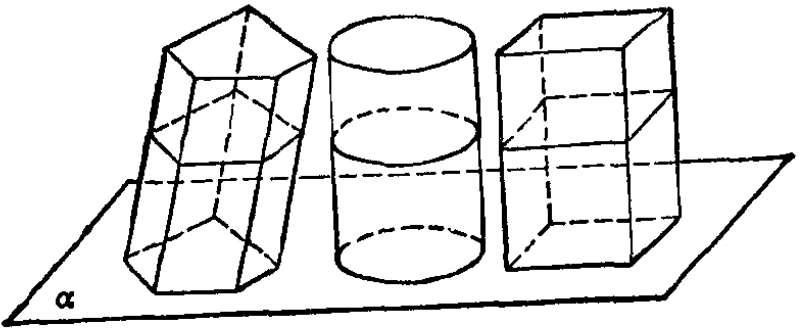
\includegraphics[width=9cm]{../pic/ltjh-ch2-60.png}
    \caption{}\label{fig:ltjh-2-60}
\end{figure}

用和平面 $\alpha$ 平行的任意平面去截它们时,所得的截面都和它们的底面分别全等,
因而这些截面的面积都等于 $S$。 根据\hyperref[zgyl]{祖暅原理},它们的体积相等。
由于长方体的体积等于它的底面积和高的乘积,于是我们得到下面的定理:

\begin{dingli}[定理][dl:zhuti-tj]
    柱体(棱柱、圆柱)的体积等于它的底面积 $\bm{S}$ 和高 $\bm{h}$ 的积。
    \begin{center}
        \framebox[10em]{$\bm{V_\text{柱体} = Sh}$。}
     \end{center}
    \vspace*{-2.5em}即
\end{dingli}\vspace{1em}


\begin{tuilun}[推论][tl:ztdtj]
    底面半径是 $\bm{r}$,高是 $\bm{h}$ 的圆柱的体积是
    $$ \bm{V_\text{圆柱} = \pi r^2h} \juhao $$
\end{tuilun}


\liti 有一堆相同规格的六角螺帽毛坯(图 \ref{fig:ltjh-2-61})共重 5.8 kg。
已知底面六边形的边长是 12 mm,高是 10 mm,内孔直径是 10 mm。
问约有毛坯多少个(铁的比重是 $7.8 \, \kmlflm$)。

\jie 六角螺帽毛坯的体积是一个正六棱柱的体积与一个圆柱的体积的差。

\begin{wrapfigure}[5]{r}{5.5cm}
    \centering
    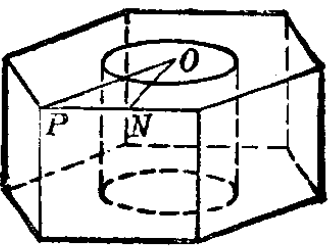
\includegraphics[width=4.5cm]{../pic/ltjh-ch2-61.png}
    \caption{}\label{fig:ltjh-2-61}
\end{wrapfigure}

$V_\text{正六俊柱} = \dfrac{\sqrt{3}}{4} \times 12^2 \times 6 \times 10 \approx 3.74 \times 10^3 \;(\lfhm)$,

$V_\text{圆柱} = 3.14 \times \left(\dfrac{10}{2}\right)^2 \times 10 \approx 0.785 \times 10^3 \; (\lfhm)$。

毛坯的体积

$\begin{aligned}
    V &= 3.74 \times 10^3 - 0.785 \times 10^3 \\
      &\approx 2.96 \times 10^3 \; (\lfhm) = 2.96 \; (\lflm) \juhao
\end{aligned}$

$5.8 \times 10^3 \div (7.8 \times 2.96) \approx 2.5 \times 10^2 \; (\text{个})$。

答: 这堆毛坯约有 250 个。



\liti 三棱柱的底面是 $\triangle ABC$,$AB = 13$ cm, $BC = 5$ cm,$CA = 12$ cm,
侧棱 $AA'$ 的长是 $20\;\limi$,如果侧棱 $AA'$ 与底面所成的角是 $60^\circ$,求这个三棱柱的体积。

\begin{wrapfigure}[5]{r}{5.5cm}
    \centering
    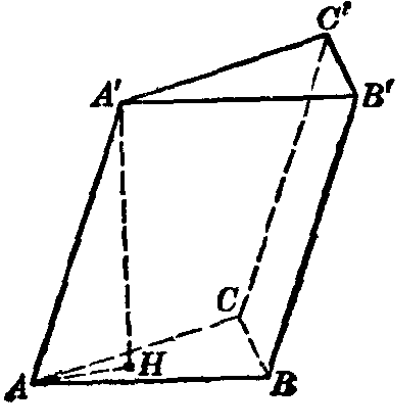
\includegraphics[width=5.5cm]{../pic/ltjh-ch2-62.png}
    \caption{}\label{fig:ltjh-2-62}
\end{wrapfigure}

\jie 设 $A'$ 在平面 $ABC$ 上的射影为 $H$。 则 $A'H$ 是棱柱的高,
$\angle A'AH = 60^\circ$ (图 \ref{fig:ltjh-2-62})。


在 $Rt \triangle A'AH$ 中,

$\because$ \quad $AA' = 20$,

$\therefore$ \quad $A'H = AA' \sin 60^\circ = 10\sqrt{3}$。

在 $\triangle ABC$ 中, $AB = 13$, $BC = 5$, $CA = 12$,

$\because$ \quad $AB^2 = BC^2 + CA^2$,

$\therefore$ \quad $\angle C = 90^\circ$。

$\therefore$ \quad $S_{\triangle ABC} = \exdfrac{1}{2} BC \cdot CA = 30 \; (\pflm)$。

\hspace*{-2em}根据柱体的体积公式,得

$V = Sh = 30 \times 10\sqrt{3} = 300\sqrt{3} \; (\lflm)$。


\begin{lianxi}

\xiaoti{一个正方体和一个圆柱等高,并且侧面积相等。比较它们的体积哪个大?大多少?}

\xiaoti{一个直平行六面体的侧棱长 9 cm,底面两条相邻边的长是 7 cm 和 11 cm,夹角为 $45^\circ$。 求它的体积。}

\end{lianxi}

\end{enhancedline}

